% ============================================================================
% FL-EHDS Paper for FLICS 2026
% IEEE Conference Format
% ============================================================================

\documentclass[conference]{IEEEtran}

% ===== PACKAGES =====
\usepackage{cite}
\usepackage{amsmath,amssymb,amsfonts}
\usepackage{graphicx}
\usepackage{textcomp}
\usepackage{xcolor}
\usepackage{booktabs}
\usepackage{hyperref}

% TikZ for vector figures
\usepackage{tikz}
\usetikzlibrary{shapes.geometric, arrows.meta, positioning, fit, backgrounds, calc}

% ===== DOCUMENT =====
\begin{document}

\title{FL-EHDS: A Privacy-Preserving Federated Learning Framework for the European Health Data Space}

\author{
    \IEEEauthorblockN{Fabio Liberti}
    \IEEEauthorblockA{
        Department of Computer Science\\
        Universitas Mercatorum, Rome, Italy\\
        fabio.liberti@unimercatorum.it
    }
}

\maketitle

% ============================================================================
% ABSTRACT
% ============================================================================
\begin{abstract}
The European Health Data Space (EHDS), effective March 2025, mandates cross-border health data analytics while preserving privacy. Federated Learning (FL) emerges as the key enabling technology, yet a systematic evidence synthesis reveals critical gaps: only 23\% of FL implementations achieve production deployment, with hardware heterogeneity (78\%) and non-IID data (67\%) as dominant barriers. Legal uncertainties regarding gradient data status under GDPR remain unresolved. We present FL-EHDS, a three-layer compliance framework integrating governance mechanisms (HDABs, data permits), FL orchestration (aggregation within Secure Processing Environments), and data holder components. The framework maps evidence-based barriers to specific mitigation strategies and provides compliance checkpoints aligned with EHDS requirements. We contribute: (1) first systematic barrier taxonomy for FL in EHDS contexts; (2) a reference architecture addressing identified gaps; (3) an implementation roadmap for the 2025-2031 transition period.
\end{abstract}

\begin{IEEEkeywords}
Federated Learning, European Health Data Space, Privacy-Preserving Technologies, GDPR, Health Data Governance
\end{IEEEkeywords}

% ============================================================================
% 1. INTRODUCTION
% ============================================================================
\section{Introduction}
\label{sec:introduction}

The European Health Data Space (EHDS), established by Regulation (EU) 2025/327, represents the EU's most ambitious initiative for cross-border health data governance~\cite{eu2025ehds}. The regulation creates a dual framework: primary use through MyHealth@EU for patient care, and secondary use through HealthData@EU for research and innovation.

\subsection{The Technology-Governance Divide}

Federated Learning (FL) emerges as the theoretically ideal solution---the model travels to data rather than centralizing sensitive records~\cite{rieke2020future}. However, recent evidence reveals a sobering gap: only 23\% of FL implementations achieve sustained production deployment~\cite{frohlich2025reality}. Technical barriers including hardware heterogeneity (78\%) and non-IID data challenges (67\%) persist. Legal uncertainties regarding gradient data status under GDPR remain unresolved~\cite{quinn2024gdpr}.

\subsection{Contributions}

This paper makes three contributions:
\begin{enumerate}
    \item \textbf{Barrier Taxonomy}: Evidence synthesis of FL barriers specific to EHDS (47 documents, PRISMA methodology).
    \item \textbf{FL-EHDS Framework}: Three-layer reference architecture with compliance checkpoints.
    \item \textbf{Implementation Roadmap}: Prioritized actions for the 2025-2031 transition.
\end{enumerate}

% ============================================================================
% 2. BACKGROUND
% ============================================================================
\section{Background}
\label{sec:background}

\subsection{European Health Data Space}

The EHDS establishes Health Data Access Bodies (HDABs) in each Member State to authorize secondary use through data permits. Article 53 enumerates permitted purposes; Article 71 introduces opt-out mechanisms~\cite{staunton2024ethical}. Table~\ref{tab:timeline} shows the implementation timeline.

\begin{table}[htbp]
\caption{EHDS Implementation Timeline}
\label{tab:timeline}
\centering
\small
\begin{tabular}{lll}
\toprule
\textbf{Date} & \textbf{Milestone} & \textbf{FL Relevance} \\
\midrule
Mar 2025 & Entry into force & Framework active \\
Mar 2027 & Delegated acts & Legal clarification \\
Mar 2029 & Secondary use & FL operational \\
Mar 2031 & Sensitive data & Genetic, imaging \\
\bottomrule
\end{tabular}
\end{table}

\subsection{Federated Learning Fundamentals}

FL inverts the traditional paradigm: rather than centralizing data, the model travels to distributed sources~\cite{mcmahan2017communication}. Local training produces gradients; these are aggregated centrally and redistributed~\cite{kairouz2021advances}. Known challenges include non-IID distributions~\cite{li2020federated}, and privacy attacks~\cite{zhu2019deep,shokri2017membership}.

% ============================================================================
% 3. FL-EHDS FRAMEWORK
% ============================================================================
\section{FL-EHDS Framework}
\label{sec:framework}

We present FL-EHDS, a three-layer compliance framework for EHDS cross-border analytics.

\subsection{Architecture Overview}

Fig.~\ref{fig:architecture} illustrates the architecture comprising:
\begin{itemize}
    \item \textbf{Layer 1 (Governance)}: HDAB integration, data permits, opt-out registry.
    \item \textbf{Layer 2 (Orchestration)}: Aggregation within SPEs, privacy and compliance modules.
    \item \textbf{Layer 3 (Data Holders)}: Local training, FHIR preprocessing.
\end{itemize}

% ===== INCLUDE FIGURE FROM figures/ FOLDER =====
% fig2-fl-ehds-architecture.tex
% FL-EHDS Three-Layer Architecture Diagram
% Grayscale version for IEEE publication
% To be placed in figures/ folder and included via % fig2-fl-ehds-architecture.tex
% FL-EHDS Three-Layer Architecture Diagram
% Grayscale version for IEEE publication
% To be placed in figures/ folder and included via % fig2-fl-ehds-architecture.tex
% FL-EHDS Three-Layer Architecture Diagram
% Grayscale version for IEEE publication
% To be placed in figures/ folder and included via \input{figures/fig2-fl-ehds-architecture}

\begin{figure*}[htbp]
\centering
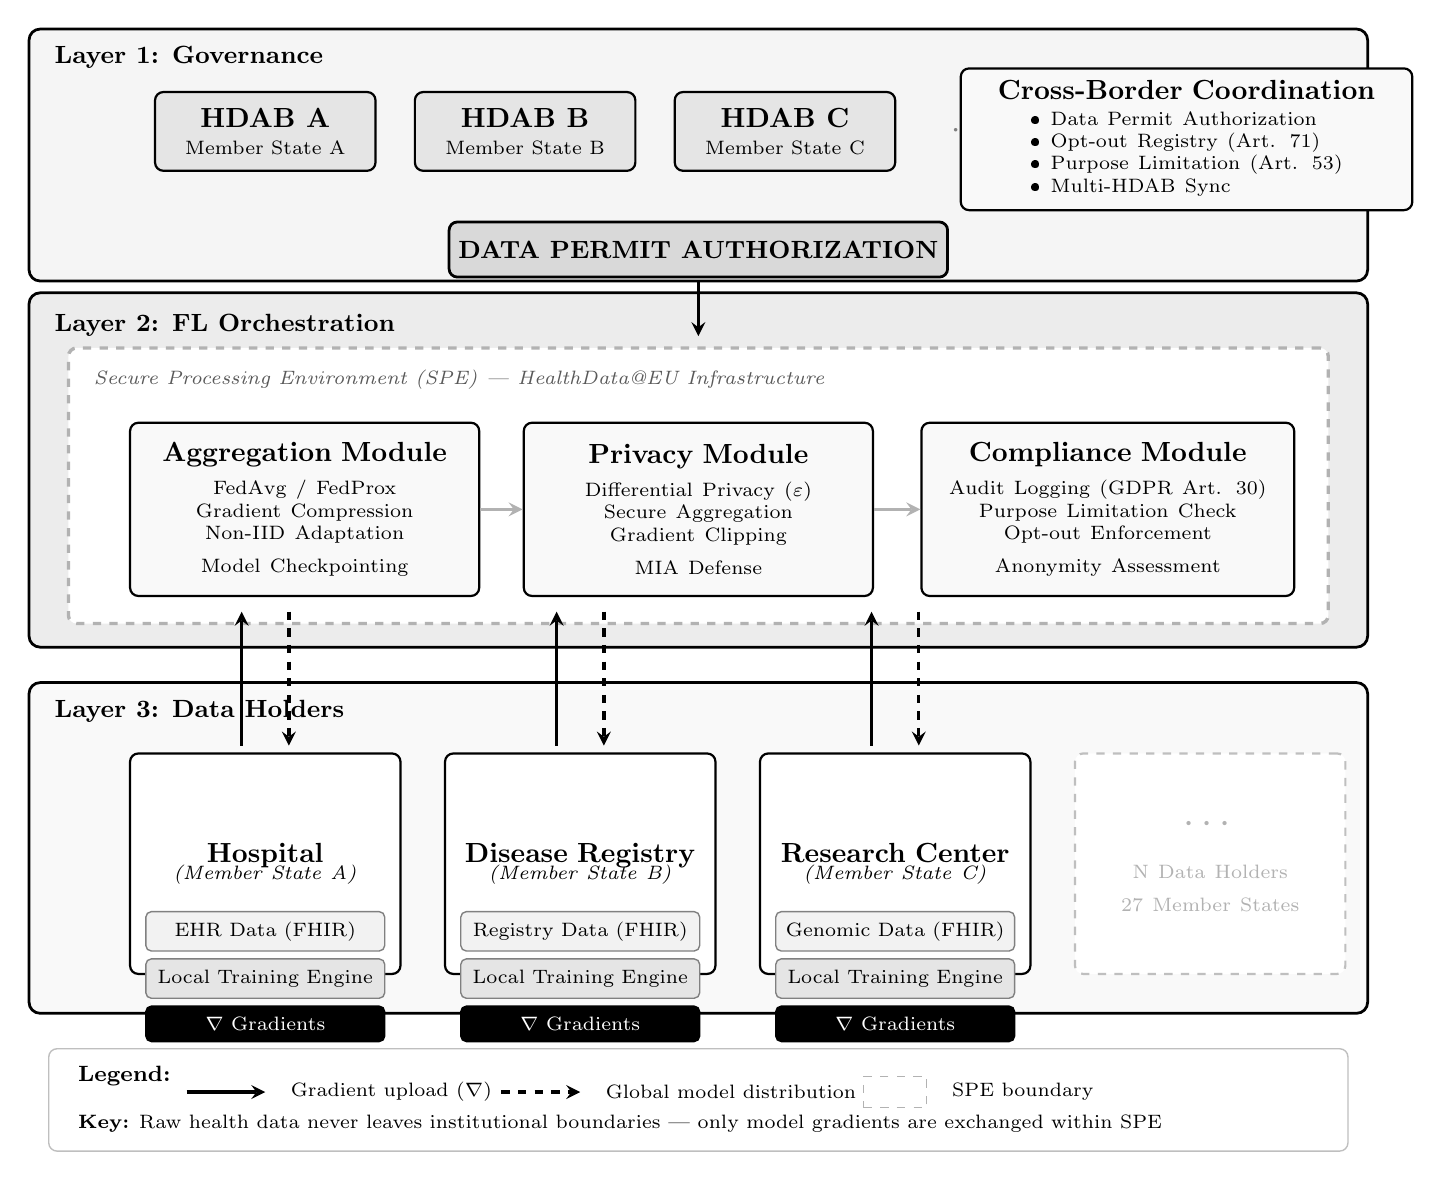
\begin{tikzpicture}[
    % Styles
    layer/.style={rectangle, rounded corners=4pt, minimum width=17cm, draw=black, line width=1pt},
    module/.style={rectangle, rounded corners=3pt, draw=black, line width=0.8pt, fill=white, minimum height=2.2cm, text width=4.2cm, align=center},
    hdab/.style={rectangle, rounded corners=3pt, draw=black, line width=0.8pt, fill=gray!20, minimum height=1cm, minimum width=2.8cm, align=center},
    dataholder/.style={rectangle, rounded corners=3pt, draw=black, line width=0.8pt, fill=white, minimum height=2.8cm, text width=3.2cm, align=center},
    databox/.style={rectangle, rounded corners=2pt, draw=gray, line width=0.5pt, fill=gray!10, minimum height=0.5cm, text width=2.8cm, align=center, font=\scriptsize},
    gradientbox/.style={rectangle, rounded corners=2pt, draw=black, line width=0.5pt, fill=black, minimum height=0.45cm, text width=2.8cm, align=center, font=\scriptsize\color{white}},
    arrow/.style={->, >=stealth, line width=1.2pt},
    dashedarrow/.style={->, >=stealth, line width=1.2pt, dashed},
    label/.style={font=\footnotesize},
    title/.style={font=\small\bfseries},
    subtitle/.style={font=\scriptsize\itshape, text=gray!70!black},
]

% ===== LAYER 1: GOVERNANCE =====
\node[layer, fill=gray!8, minimum height=3.2cm] (layer1) at (0, 8) {};
\node[title, anchor=north west] at (-8.3, 9.5) {Layer 1: Governance};

% HDABs
\node[hdab] (hdabA) at (-5.5, 8.3) {\textbf{HDAB A}\\[-2pt]\scriptsize Member State A};
\node[hdab] (hdabB) at (-2.2, 8.3) {\textbf{HDAB B}\\[-2pt]\scriptsize Member State B};
\node[hdab] (hdabC) at (1.1, 8.3) {\textbf{HDAB C}\\[-2pt]\scriptsize Member State C};
\node[font=\large, text=gray] at (3.5, 8.3) {$\cdots$};

% Coordination box
\node[module, minimum height=1.8cm, text width=5.5cm, fill=gray!5] (coord) at (6.2, 8.2) {
    \textbf{Cross-Border Coordination}\\[3pt]
    \scriptsize
    \begin{tabular}{@{}l@{}}
    • Data Permit Authorization\\
    • Opt-out Registry (Art. 71)\\
    • Purpose Limitation (Art. 53)\\
    • Multi-HDAB Sync
    \end{tabular}
};

% Data Permit box
\node[rectangle, rounded corners=3pt, draw=black, line width=1pt, fill=gray!30, minimum height=0.7cm, minimum width=5cm] (permit) at (0, 6.8) {\small\textbf{DATA PERMIT AUTHORIZATION}};

% ===== LAYER 2: FL ORCHESTRATION =====
\node[layer, fill=gray!15, minimum height=4.5cm] (layer2) at (0, 4) {};
\node[title, anchor=north west] at (-8.3, 6.1) {Layer 2: FL Orchestration};

% SPE boundary
\node[rectangle, rounded corners=3pt, draw=gray!60, line width=1.2pt, dashed, minimum width=16cm, minimum height=3.5cm, fill=white] (spe) at (0, 3.8) {};
\node[subtitle, anchor=north west] at (-7.8, 5.4) {Secure Processing Environment (SPE) — HealthData@EU Infrastructure};

% Modules
\node[module, fill=gray!5] (agg) at (-5, 3.5) {
    \textbf{Aggregation Module}\\[4pt]
    \scriptsize
    FedAvg / FedProx\\
    Gradient Compression\\
    Non-IID Adaptation\\
    Model Checkpointing
};

\node[module, fill=gray!5] (priv) at (0, 3.5) {
    \textbf{Privacy Module}\\[4pt]
    \scriptsize
    Differential Privacy ($\varepsilon$)\\
    Secure Aggregation\\
    Gradient Clipping\\
    MIA Defense
};

\node[module, fill=gray!5, text width=4.5cm] (comp) at (5.2, 3.5) {
    \textbf{Compliance Module}\\[4pt]
    \scriptsize
    Audit Logging (GDPR Art. 30)\\
    Purpose Limitation Check\\
    Opt-out Enforcement\\
    Anonymity Assessment
};

% Arrows between modules
\draw[arrow, gray!60] (agg.east) -- (priv.west);
\draw[arrow, gray!60] (priv.east) -- (comp.west);

% ===== LAYER 3: DATA HOLDERS =====
\node[layer, fill=gray!5, minimum height=4.2cm] (layer3) at (0, -0.8) {};
\node[title, anchor=north west] at (-8.3, 1.2) {Layer 3: Data Holders};

% Data holders
\node[dataholder] (hosp) at (-5.5, -1) {
    \textbf{Hospital}\\[-2pt]
    \scriptsize\textit{(Member State A)}\\[6pt]
};
\node[databox, anchor=north] at (-5.5, -1.6) {EHR Data (FHIR)};
\node[databox, anchor=north, fill=gray!20] at (-5.5, -2.2) {Local Training Engine};
\node[gradientbox, anchor=north] at (-5.5, -2.8) {$\nabla$ Gradients};

\node[dataholder] (reg) at (-1.5, -1) {
    \textbf{Disease Registry}\\[-2pt]
    \scriptsize\textit{(Member State B)}\\[6pt]
};
\node[databox, anchor=north] at (-1.5, -1.6) {Registry Data (FHIR)};
\node[databox, anchor=north, fill=gray!20] at (-1.5, -2.2) {Local Training Engine};
\node[gradientbox, anchor=north] at (-1.5, -2.8) {$\nabla$ Gradients};

\node[dataholder] (res) at (2.5, -1) {
    \textbf{Research Center}\\[-2pt]
    \scriptsize\textit{(Member State C)}\\[6pt]
};
\node[databox, anchor=north] at (2.5, -1.6) {Genomic Data (FHIR)};
\node[databox, anchor=north, fill=gray!20] at (2.5, -2.2) {Local Training Engine};
\node[gradientbox, anchor=north] at (2.5, -2.8) {$\nabla$ Gradients};

% More nodes indicator
\node[dataholder, draw=gray!50, dashed, text=gray!60] (more) at (6.5, -1) {
    \Large$\cdots$\\[8pt]
    \scriptsize N Data Holders\\
    27 Member States
};

% ===== DATA FLOW ARROWS =====
% Gradients up (solid)
\draw[arrow] (-5.8, 0.5) -- (-5.8, 2.2) node[midway, left, font=\tiny] {};
\draw[arrow] (-1.8, 0.5) -- (-1.8, 2.2);
\draw[arrow] (2.2, 0.5) -- (2.2, 2.2);

% Model down (dashed)
\draw[dashedarrow] (-5.2, 2.2) -- (-5.2, 0.5);
\draw[dashedarrow] (-1.2, 2.2) -- (-1.2, 0.5);
\draw[dashedarrow] (2.8, 2.2) -- (2.8, 0.5);

% Layer 1 to Layer 2
\draw[arrow] (0, 6.4) -- (0, 5.7);

% ===== LEGEND =====
\node[rectangle, rounded corners=3pt, draw=gray!50, line width=0.5pt, fill=white, minimum width=16.5cm, minimum height=1.3cm] at (0, -4) {};
\node[font=\footnotesize\bfseries, anchor=west] at (-8, -3.7) {Legend:};

% Gradient arrow
\draw[arrow] (-6.5, -3.9) -- (-5.5, -3.9);
\node[font=\scriptsize, anchor=west] at (-5.3, -3.9) {Gradient upload ($\nabla$)};

% Model arrow  
\draw[dashedarrow] (-2.5, -3.9) -- (-1.5, -3.9);
\node[font=\scriptsize, anchor=west] at (-1.3, -3.9) {Global model distribution};

% SPE
\node[rectangle, draw=gray!60, dashed, minimum width=0.8cm, minimum height=0.4cm] at (2.5, -3.9) {};
\node[font=\scriptsize, anchor=west] at (3.1, -3.9) {SPE boundary};

% Key principle
\node[font=\scriptsize, anchor=west] at (-8, -4.3) {\textbf{Key:} Raw health data never leaves institutional boundaries — only model gradients are exchanged within SPE};

\end{tikzpicture}
\caption{FL-EHDS three-layer compliance framework architecture. Layer~1 (Governance) integrates Health Data Access Bodies for cross-border data permit authorization and opt-out registry consultation per Article~71. Layer~2 (FL Orchestration) operates within a Secure Processing Environment, implementing gradient aggregation with FedAvg/FedProx, privacy protection via differential privacy and secure aggregation, and GDPR-compliant audit logging. Layer~3 (Data Holders) maintains raw data within institutional boundaries across 27 Member States; only gradients ($\nabla$) are transmitted upward while global model parameters flow downward.}
\label{fig:architecture}
\end{figure*}


\begin{figure*}[htbp]
\centering
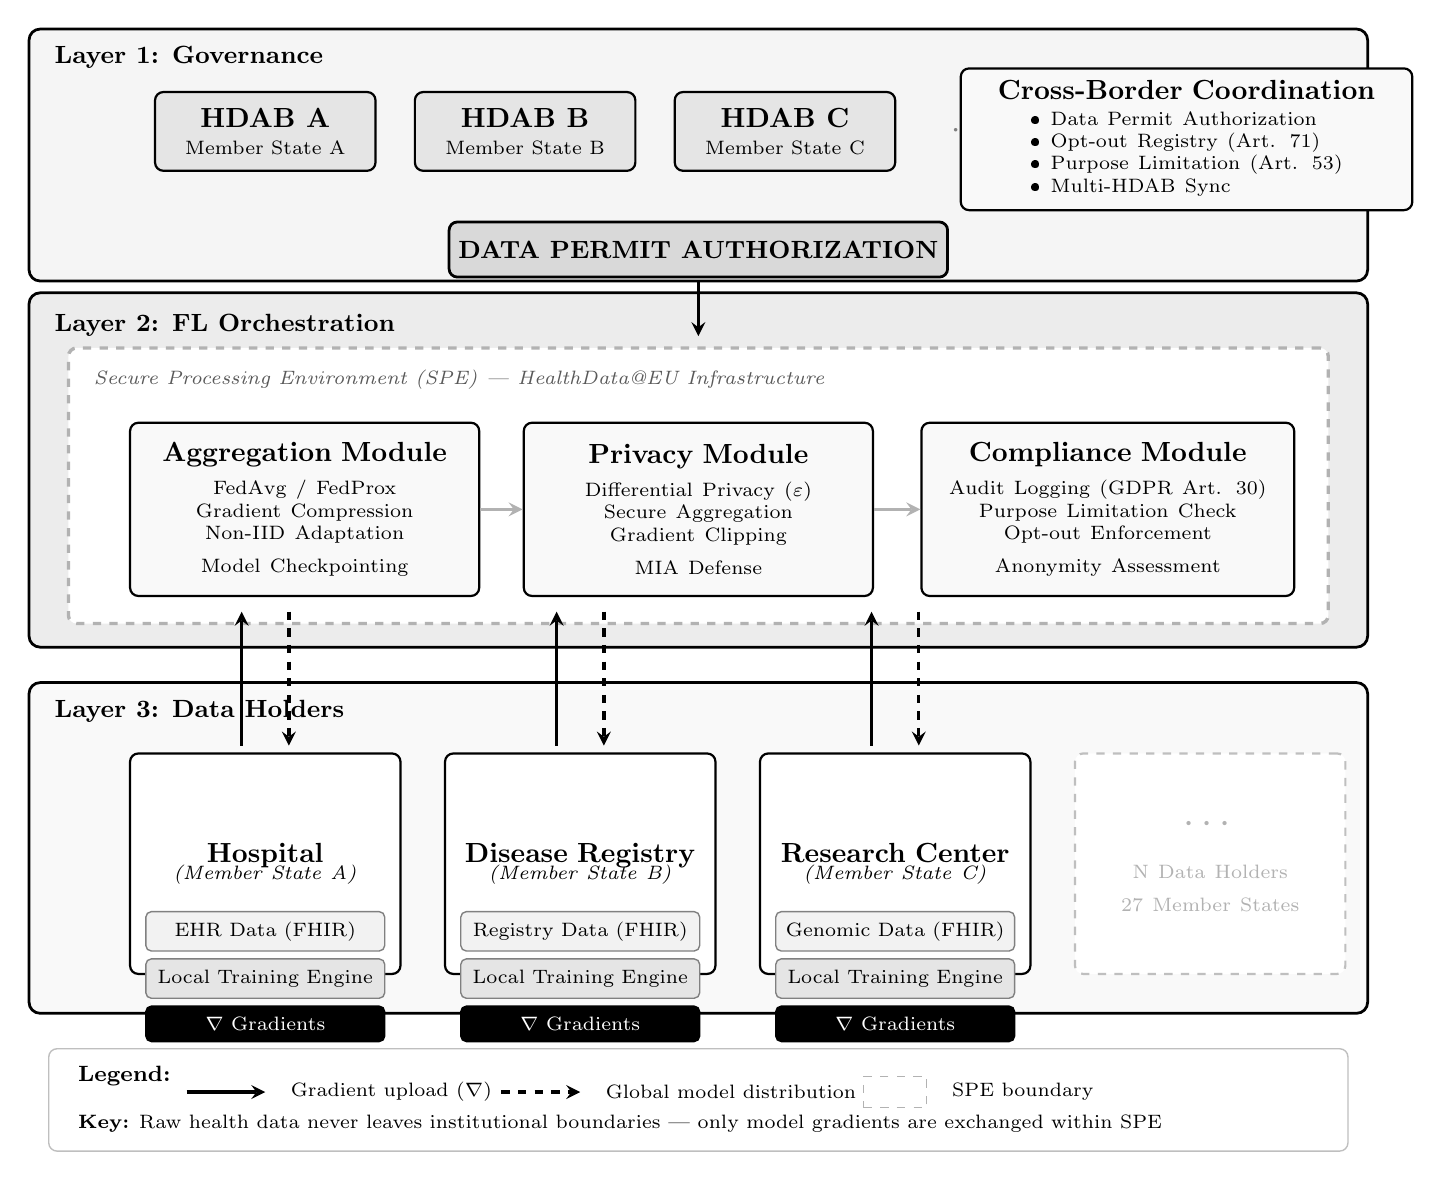
\begin{tikzpicture}[
    % Styles
    layer/.style={rectangle, rounded corners=4pt, minimum width=17cm, draw=black, line width=1pt},
    module/.style={rectangle, rounded corners=3pt, draw=black, line width=0.8pt, fill=white, minimum height=2.2cm, text width=4.2cm, align=center},
    hdab/.style={rectangle, rounded corners=3pt, draw=black, line width=0.8pt, fill=gray!20, minimum height=1cm, minimum width=2.8cm, align=center},
    dataholder/.style={rectangle, rounded corners=3pt, draw=black, line width=0.8pt, fill=white, minimum height=2.8cm, text width=3.2cm, align=center},
    databox/.style={rectangle, rounded corners=2pt, draw=gray, line width=0.5pt, fill=gray!10, minimum height=0.5cm, text width=2.8cm, align=center, font=\scriptsize},
    gradientbox/.style={rectangle, rounded corners=2pt, draw=black, line width=0.5pt, fill=black, minimum height=0.45cm, text width=2.8cm, align=center, font=\scriptsize\color{white}},
    arrow/.style={->, >=stealth, line width=1.2pt},
    dashedarrow/.style={->, >=stealth, line width=1.2pt, dashed},
    label/.style={font=\footnotesize},
    title/.style={font=\small\bfseries},
    subtitle/.style={font=\scriptsize\itshape, text=gray!70!black},
]

% ===== LAYER 1: GOVERNANCE =====
\node[layer, fill=gray!8, minimum height=3.2cm] (layer1) at (0, 8) {};
\node[title, anchor=north west] at (-8.3, 9.5) {Layer 1: Governance};

% HDABs
\node[hdab] (hdabA) at (-5.5, 8.3) {\textbf{HDAB A}\\[-2pt]\scriptsize Member State A};
\node[hdab] (hdabB) at (-2.2, 8.3) {\textbf{HDAB B}\\[-2pt]\scriptsize Member State B};
\node[hdab] (hdabC) at (1.1, 8.3) {\textbf{HDAB C}\\[-2pt]\scriptsize Member State C};
\node[font=\large, text=gray] at (3.5, 8.3) {$\cdots$};

% Coordination box
\node[module, minimum height=1.8cm, text width=5.5cm, fill=gray!5] (coord) at (6.2, 8.2) {
    \textbf{Cross-Border Coordination}\\[3pt]
    \scriptsize
    \begin{tabular}{@{}l@{}}
    • Data Permit Authorization\\
    • Opt-out Registry (Art. 71)\\
    • Purpose Limitation (Art. 53)\\
    • Multi-HDAB Sync
    \end{tabular}
};

% Data Permit box
\node[rectangle, rounded corners=3pt, draw=black, line width=1pt, fill=gray!30, minimum height=0.7cm, minimum width=5cm] (permit) at (0, 6.8) {\small\textbf{DATA PERMIT AUTHORIZATION}};

% ===== LAYER 2: FL ORCHESTRATION =====
\node[layer, fill=gray!15, minimum height=4.5cm] (layer2) at (0, 4) {};
\node[title, anchor=north west] at (-8.3, 6.1) {Layer 2: FL Orchestration};

% SPE boundary
\node[rectangle, rounded corners=3pt, draw=gray!60, line width=1.2pt, dashed, minimum width=16cm, minimum height=3.5cm, fill=white] (spe) at (0, 3.8) {};
\node[subtitle, anchor=north west] at (-7.8, 5.4) {Secure Processing Environment (SPE) — HealthData@EU Infrastructure};

% Modules
\node[module, fill=gray!5] (agg) at (-5, 3.5) {
    \textbf{Aggregation Module}\\[4pt]
    \scriptsize
    FedAvg / FedProx\\
    Gradient Compression\\
    Non-IID Adaptation\\
    Model Checkpointing
};

\node[module, fill=gray!5] (priv) at (0, 3.5) {
    \textbf{Privacy Module}\\[4pt]
    \scriptsize
    Differential Privacy ($\varepsilon$)\\
    Secure Aggregation\\
    Gradient Clipping\\
    MIA Defense
};

\node[module, fill=gray!5, text width=4.5cm] (comp) at (5.2, 3.5) {
    \textbf{Compliance Module}\\[4pt]
    \scriptsize
    Audit Logging (GDPR Art. 30)\\
    Purpose Limitation Check\\
    Opt-out Enforcement\\
    Anonymity Assessment
};

% Arrows between modules
\draw[arrow, gray!60] (agg.east) -- (priv.west);
\draw[arrow, gray!60] (priv.east) -- (comp.west);

% ===== LAYER 3: DATA HOLDERS =====
\node[layer, fill=gray!5, minimum height=4.2cm] (layer3) at (0, -0.8) {};
\node[title, anchor=north west] at (-8.3, 1.2) {Layer 3: Data Holders};

% Data holders
\node[dataholder] (hosp) at (-5.5, -1) {
    \textbf{Hospital}\\[-2pt]
    \scriptsize\textit{(Member State A)}\\[6pt]
};
\node[databox, anchor=north] at (-5.5, -1.6) {EHR Data (FHIR)};
\node[databox, anchor=north, fill=gray!20] at (-5.5, -2.2) {Local Training Engine};
\node[gradientbox, anchor=north] at (-5.5, -2.8) {$\nabla$ Gradients};

\node[dataholder] (reg) at (-1.5, -1) {
    \textbf{Disease Registry}\\[-2pt]
    \scriptsize\textit{(Member State B)}\\[6pt]
};
\node[databox, anchor=north] at (-1.5, -1.6) {Registry Data (FHIR)};
\node[databox, anchor=north, fill=gray!20] at (-1.5, -2.2) {Local Training Engine};
\node[gradientbox, anchor=north] at (-1.5, -2.8) {$\nabla$ Gradients};

\node[dataholder] (res) at (2.5, -1) {
    \textbf{Research Center}\\[-2pt]
    \scriptsize\textit{(Member State C)}\\[6pt]
};
\node[databox, anchor=north] at (2.5, -1.6) {Genomic Data (FHIR)};
\node[databox, anchor=north, fill=gray!20] at (2.5, -2.2) {Local Training Engine};
\node[gradientbox, anchor=north] at (2.5, -2.8) {$\nabla$ Gradients};

% More nodes indicator
\node[dataholder, draw=gray!50, dashed, text=gray!60] (more) at (6.5, -1) {
    \Large$\cdots$\\[8pt]
    \scriptsize N Data Holders\\
    27 Member States
};

% ===== DATA FLOW ARROWS =====
% Gradients up (solid)
\draw[arrow] (-5.8, 0.5) -- (-5.8, 2.2) node[midway, left, font=\tiny] {};
\draw[arrow] (-1.8, 0.5) -- (-1.8, 2.2);
\draw[arrow] (2.2, 0.5) -- (2.2, 2.2);

% Model down (dashed)
\draw[dashedarrow] (-5.2, 2.2) -- (-5.2, 0.5);
\draw[dashedarrow] (-1.2, 2.2) -- (-1.2, 0.5);
\draw[dashedarrow] (2.8, 2.2) -- (2.8, 0.5);

% Layer 1 to Layer 2
\draw[arrow] (0, 6.4) -- (0, 5.7);

% ===== LEGEND =====
\node[rectangle, rounded corners=3pt, draw=gray!50, line width=0.5pt, fill=white, minimum width=16.5cm, minimum height=1.3cm] at (0, -4) {};
\node[font=\footnotesize\bfseries, anchor=west] at (-8, -3.7) {Legend:};

% Gradient arrow
\draw[arrow] (-6.5, -3.9) -- (-5.5, -3.9);
\node[font=\scriptsize, anchor=west] at (-5.3, -3.9) {Gradient upload ($\nabla$)};

% Model arrow  
\draw[dashedarrow] (-2.5, -3.9) -- (-1.5, -3.9);
\node[font=\scriptsize, anchor=west] at (-1.3, -3.9) {Global model distribution};

% SPE
\node[rectangle, draw=gray!60, dashed, minimum width=0.8cm, minimum height=0.4cm] at (2.5, -3.9) {};
\node[font=\scriptsize, anchor=west] at (3.1, -3.9) {SPE boundary};

% Key principle
\node[font=\scriptsize, anchor=west] at (-8, -4.3) {\textbf{Key:} Raw health data never leaves institutional boundaries — only model gradients are exchanged within SPE};

\end{tikzpicture}
\caption{FL-EHDS three-layer compliance framework architecture. Layer~1 (Governance) integrates Health Data Access Bodies for cross-border data permit authorization and opt-out registry consultation per Article~71. Layer~2 (FL Orchestration) operates within a Secure Processing Environment, implementing gradient aggregation with FedAvg/FedProx, privacy protection via differential privacy and secure aggregation, and GDPR-compliant audit logging. Layer~3 (Data Holders) maintains raw data within institutional boundaries across 27 Member States; only gradients ($\nabla$) are transmitted upward while global model parameters flow downward.}
\label{fig:architecture}
\end{figure*}


\begin{figure*}[htbp]
\centering
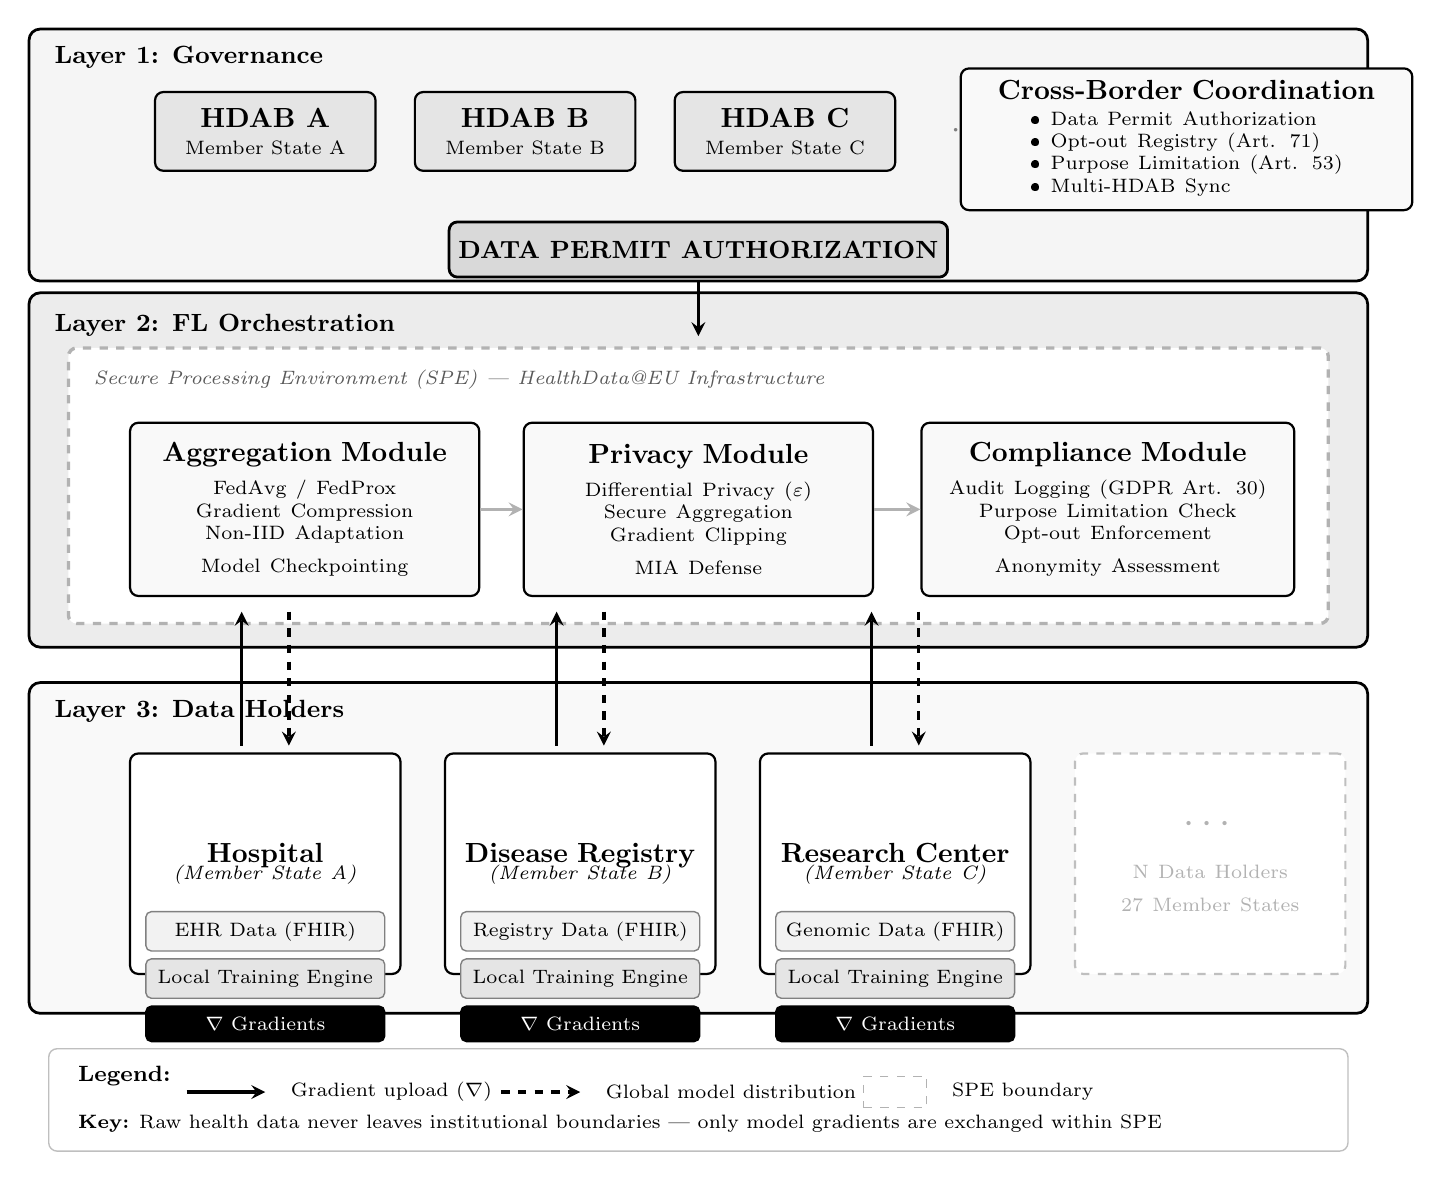
\begin{tikzpicture}[
    % Styles
    layer/.style={rectangle, rounded corners=4pt, minimum width=17cm, draw=black, line width=1pt},
    module/.style={rectangle, rounded corners=3pt, draw=black, line width=0.8pt, fill=white, minimum height=2.2cm, text width=4.2cm, align=center},
    hdab/.style={rectangle, rounded corners=3pt, draw=black, line width=0.8pt, fill=gray!20, minimum height=1cm, minimum width=2.8cm, align=center},
    dataholder/.style={rectangle, rounded corners=3pt, draw=black, line width=0.8pt, fill=white, minimum height=2.8cm, text width=3.2cm, align=center},
    databox/.style={rectangle, rounded corners=2pt, draw=gray, line width=0.5pt, fill=gray!10, minimum height=0.5cm, text width=2.8cm, align=center, font=\scriptsize},
    gradientbox/.style={rectangle, rounded corners=2pt, draw=black, line width=0.5pt, fill=black, minimum height=0.45cm, text width=2.8cm, align=center, font=\scriptsize\color{white}},
    arrow/.style={->, >=stealth, line width=1.2pt},
    dashedarrow/.style={->, >=stealth, line width=1.2pt, dashed},
    label/.style={font=\footnotesize},
    title/.style={font=\small\bfseries},
    subtitle/.style={font=\scriptsize\itshape, text=gray!70!black},
]

% ===== LAYER 1: GOVERNANCE =====
\node[layer, fill=gray!8, minimum height=3.2cm] (layer1) at (0, 8) {};
\node[title, anchor=north west] at (-8.3, 9.5) {Layer 1: Governance};

% HDABs
\node[hdab] (hdabA) at (-5.5, 8.3) {\textbf{HDAB A}\\[-2pt]\scriptsize Member State A};
\node[hdab] (hdabB) at (-2.2, 8.3) {\textbf{HDAB B}\\[-2pt]\scriptsize Member State B};
\node[hdab] (hdabC) at (1.1, 8.3) {\textbf{HDAB C}\\[-2pt]\scriptsize Member State C};
\node[font=\large, text=gray] at (3.5, 8.3) {$\cdots$};

% Coordination box
\node[module, minimum height=1.8cm, text width=5.5cm, fill=gray!5] (coord) at (6.2, 8.2) {
    \textbf{Cross-Border Coordination}\\[3pt]
    \scriptsize
    \begin{tabular}{@{}l@{}}
    • Data Permit Authorization\\
    • Opt-out Registry (Art. 71)\\
    • Purpose Limitation (Art. 53)\\
    • Multi-HDAB Sync
    \end{tabular}
};

% Data Permit box
\node[rectangle, rounded corners=3pt, draw=black, line width=1pt, fill=gray!30, minimum height=0.7cm, minimum width=5cm] (permit) at (0, 6.8) {\small\textbf{DATA PERMIT AUTHORIZATION}};

% ===== LAYER 2: FL ORCHESTRATION =====
\node[layer, fill=gray!15, minimum height=4.5cm] (layer2) at (0, 4) {};
\node[title, anchor=north west] at (-8.3, 6.1) {Layer 2: FL Orchestration};

% SPE boundary
\node[rectangle, rounded corners=3pt, draw=gray!60, line width=1.2pt, dashed, minimum width=16cm, minimum height=3.5cm, fill=white] (spe) at (0, 3.8) {};
\node[subtitle, anchor=north west] at (-7.8, 5.4) {Secure Processing Environment (SPE) — HealthData@EU Infrastructure};

% Modules
\node[module, fill=gray!5] (agg) at (-5, 3.5) {
    \textbf{Aggregation Module}\\[4pt]
    \scriptsize
    FedAvg / FedProx\\
    Gradient Compression\\
    Non-IID Adaptation\\
    Model Checkpointing
};

\node[module, fill=gray!5] (priv) at (0, 3.5) {
    \textbf{Privacy Module}\\[4pt]
    \scriptsize
    Differential Privacy ($\varepsilon$)\\
    Secure Aggregation\\
    Gradient Clipping\\
    MIA Defense
};

\node[module, fill=gray!5, text width=4.5cm] (comp) at (5.2, 3.5) {
    \textbf{Compliance Module}\\[4pt]
    \scriptsize
    Audit Logging (GDPR Art. 30)\\
    Purpose Limitation Check\\
    Opt-out Enforcement\\
    Anonymity Assessment
};

% Arrows between modules
\draw[arrow, gray!60] (agg.east) -- (priv.west);
\draw[arrow, gray!60] (priv.east) -- (comp.west);

% ===== LAYER 3: DATA HOLDERS =====
\node[layer, fill=gray!5, minimum height=4.2cm] (layer3) at (0, -0.8) {};
\node[title, anchor=north west] at (-8.3, 1.2) {Layer 3: Data Holders};

% Data holders
\node[dataholder] (hosp) at (-5.5, -1) {
    \textbf{Hospital}\\[-2pt]
    \scriptsize\textit{(Member State A)}\\[6pt]
};
\node[databox, anchor=north] at (-5.5, -1.6) {EHR Data (FHIR)};
\node[databox, anchor=north, fill=gray!20] at (-5.5, -2.2) {Local Training Engine};
\node[gradientbox, anchor=north] at (-5.5, -2.8) {$\nabla$ Gradients};

\node[dataholder] (reg) at (-1.5, -1) {
    \textbf{Disease Registry}\\[-2pt]
    \scriptsize\textit{(Member State B)}\\[6pt]
};
\node[databox, anchor=north] at (-1.5, -1.6) {Registry Data (FHIR)};
\node[databox, anchor=north, fill=gray!20] at (-1.5, -2.2) {Local Training Engine};
\node[gradientbox, anchor=north] at (-1.5, -2.8) {$\nabla$ Gradients};

\node[dataholder] (res) at (2.5, -1) {
    \textbf{Research Center}\\[-2pt]
    \scriptsize\textit{(Member State C)}\\[6pt]
};
\node[databox, anchor=north] at (2.5, -1.6) {Genomic Data (FHIR)};
\node[databox, anchor=north, fill=gray!20] at (2.5, -2.2) {Local Training Engine};
\node[gradientbox, anchor=north] at (2.5, -2.8) {$\nabla$ Gradients};

% More nodes indicator
\node[dataholder, draw=gray!50, dashed, text=gray!60] (more) at (6.5, -1) {
    \Large$\cdots$\\[8pt]
    \scriptsize N Data Holders\\
    27 Member States
};

% ===== DATA FLOW ARROWS =====
% Gradients up (solid)
\draw[arrow] (-5.8, 0.5) -- (-5.8, 2.2) node[midway, left, font=\tiny] {};
\draw[arrow] (-1.8, 0.5) -- (-1.8, 2.2);
\draw[arrow] (2.2, 0.5) -- (2.2, 2.2);

% Model down (dashed)
\draw[dashedarrow] (-5.2, 2.2) -- (-5.2, 0.5);
\draw[dashedarrow] (-1.2, 2.2) -- (-1.2, 0.5);
\draw[dashedarrow] (2.8, 2.2) -- (2.8, 0.5);

% Layer 1 to Layer 2
\draw[arrow] (0, 6.4) -- (0, 5.7);

% ===== LEGEND =====
\node[rectangle, rounded corners=3pt, draw=gray!50, line width=0.5pt, fill=white, minimum width=16.5cm, minimum height=1.3cm] at (0, -4) {};
\node[font=\footnotesize\bfseries, anchor=west] at (-8, -3.7) {Legend:};

% Gradient arrow
\draw[arrow] (-6.5, -3.9) -- (-5.5, -3.9);
\node[font=\scriptsize, anchor=west] at (-5.3, -3.9) {Gradient upload ($\nabla$)};

% Model arrow  
\draw[dashedarrow] (-2.5, -3.9) -- (-1.5, -3.9);
\node[font=\scriptsize, anchor=west] at (-1.3, -3.9) {Global model distribution};

% SPE
\node[rectangle, draw=gray!60, dashed, minimum width=0.8cm, minimum height=0.4cm] at (2.5, -3.9) {};
\node[font=\scriptsize, anchor=west] at (3.1, -3.9) {SPE boundary};

% Key principle
\node[font=\scriptsize, anchor=west] at (-8, -4.3) {\textbf{Key:} Raw health data never leaves institutional boundaries — only model gradients are exchanged within SPE};

\end{tikzpicture}
\caption{FL-EHDS three-layer compliance framework architecture. Layer~1 (Governance) integrates Health Data Access Bodies for cross-border data permit authorization and opt-out registry consultation per Article~71. Layer~2 (FL Orchestration) operates within a Secure Processing Environment, implementing gradient aggregation with FedAvg/FedProx, privacy protection via differential privacy and secure aggregation, and GDPR-compliant audit logging. Layer~3 (Data Holders) maintains raw data within institutional boundaries across 27 Member States; only gradients ($\nabla$) are transmitted upward while global model parameters flow downward.}
\label{fig:architecture}
\end{figure*}


\subsection{Layer 1: Governance Layer}

\textbf{HDAB Integration}: Standardized APIs enable automated data permit verification. Multi-HDAB synchronization coordinates cross-border studies.

\textbf{Opt-out Registry}: National registries are consulted before training, ensuring Article 71 compliance.

\subsection{Layer 2: FL Orchestration Layer}

\textbf{Aggregation Module}: FedAvg~\cite{mcmahan2017communication} with FedProx~\cite{li2020federated} for non-IID data. Gradient compression reduces communication overhead.

\textbf{Privacy Protection}: Differential privacy with $\varepsilon$-budget; gradient clipping; membership inference defense.

\textbf{Compliance}: Audit logging (GDPR Art. 30); purpose limitation enforcement.

\subsection{Layer 3: Data Holder Layer}

\textbf{Adaptive Training}: Resource-aware model partitioning for hardware heterogeneity.

\textbf{FHIR Preprocessing}: Data normalization ensures interoperability.

\textbf{Secure Communication}: Encrypted gradients; no raw data leaves institutions.

% ============================================================================
% 4. EVIDENCE SYNTHESIS
% ============================================================================
\section{Evidence Synthesis}
\label{sec:evidence}

\subsection{Technical Barriers}

Table~\ref{tab:barriers} summarizes barriers from systematic review (847 records, 47 included).

\begin{table}[htbp]
\caption{FL Implementation Barriers for EHDS}
\label{tab:barriers}
\centering
\small
\begin{tabular}{p{2.2cm}cp{2.3cm}p{1.8cm}}
\toprule
\textbf{Barrier} & \textbf{Prev.} & \textbf{Evidence} & \textbf{Mitigation} \\
\midrule
Hardware heterogeneity & 78\% & Fr\"ohlich 2025 & Adaptive engine \\
Non-IID data & 67\% & Multiple & FedProx \\
Production gap & 23\% & Fr\"ohlich 2025 & Ref. impl. \\
FHIR compliance & 34\% & Hussein 2025 & Preprocessing \\
\bottomrule
\end{tabular}
\end{table}

\subsection{Legal Uncertainties}

Three questions remain unresolved: (1) gradient data status under GDPR; (2) model anonymity thresholds; (3) controller/processor allocation in FL~\cite{quinn2024gdpr}.

\subsection{Organizational Barriers}

HDAB capacity shows Nordic countries 2-3 years ahead~\cite{tehdas2024ready}. Access timelines: 3 weeks (Finland) to 12+ months (France)~\cite{forster2025journeys}.

% ============================================================================
% 5. IMPLEMENTATION ROADMAP
% ============================================================================
\section{Implementation Roadmap}
\label{sec:roadmap}

Table~\ref{tab:roadmap} presents phased implementation.

\begin{table}[htbp]
\caption{FL-EHDS Implementation Roadmap}
\label{tab:roadmap}
\centering
\small
\begin{tabular}{llp{3.5cm}}
\toprule
\textbf{Phase} & \textbf{Timeline} & \textbf{Actions} \\
\midrule
Foundation & 2025-26 & Reference implementation; pilots \\
Clarification & 2027 & Delegated acts; legal guidance \\
Scaling & 2028-29 & Multi-MS deployment \\
Operation & 2029-31 & Full production \\
\bottomrule
\end{tabular}
\end{table}

\textbf{EU Policymakers}: Clarify gradient status in 2027 delegated acts.

\textbf{National Authorities}: Invest in HDAB capacity; staff training.

\textbf{Healthcare Organizations}: Accelerate FHIR; pilot participation.

% ============================================================================
% 6. CONCLUSIONS
% ============================================================================
\section{Conclusions}
\label{sec:conclusions}

This paper presents FL-EHDS, a three-layer framework bridging the technology-governance divide. Key finding: \textbf{legal uncertainties---not technical barriers---are the critical blocker}. The 2027 delegated acts represent a critical window; without clarification, the 2029 deadline arrives with FL adoption inhibited by uncertainty.

Future work: empirical validation through HealthData@EU pilots; citizen attitude studies; economic sustainability modeling.

% ============================================================================
% ACKNOWLEDGMENTS
% ============================================================================
\section*{Acknowledgments}
The author thanks the TEHDAS Joint Action consortium.

% ============================================================================
% REFERENCES
% ============================================================================
\bibliographystyle{IEEEtran}

\begin{thebibliography}{00}

\bibitem{eu2025ehds}
European Commission, ``Regulation (EU) 2025/327 on the European Health Data Space,'' \textit{Official Journal of the EU}, 2025.

\bibitem{rieke2020future}
N. Rieke \textit{et al.}, ``The future of digital health with federated learning,'' \textit{NPJ Digital Medicine}, vol.~3, art.~119, 2020.

\bibitem{frohlich2025reality}
H. Fr\"ohlich \textit{et al.}, ``Reality check: The aspirations of the EHDS amidst challenges in decentralized data analysis,'' \textit{JMIR}, vol.~27, e76491, 2025.

\bibitem{quinn2024gdpr}
P. Quinn \textit{et al.}, ``Will the GDPR restrain HDABs under the EHDS?'' \textit{Computer Law \& Security Review}, vol.~54, 105993, 2024.

\bibitem{staunton2024ethical}
C. Staunton \textit{et al.}, ``Ethical reflections on the EHDS,'' \textit{Eur.~J.~Human Genetics}, vol.~32, no.~5, pp.~498--505, 2024.

\bibitem{mcmahan2017communication}
B. McMahan \textit{et al.}, ``Communication-efficient learning from decentralized data,'' \textit{AISTATS}, pp.~1273--1282, 2017.

\bibitem{kairouz2021advances}
P. Kairouz \textit{et al.}, ``Advances and open problems in federated learning,'' \textit{Found.~Trends ML}, vol.~14, no.~1--2, 2021.

\bibitem{li2020federated}
T. Li \textit{et al.}, ``Federated optimization in heterogeneous networks,'' \textit{MLSys}, vol.~2, pp.~429--450, 2020.

\bibitem{zhu2019deep}
L. Zhu \textit{et al.}, ``Deep leakage from gradients,'' \textit{NeurIPS}, vol.~32, 2019.

\bibitem{shokri2017membership}
R. Shokri \textit{et al.}, ``Membership inference attacks,'' \textit{IEEE S\&P}, pp.~3--18, 2017.

\bibitem{tehdas2024ready}
TEHDAS, ``Are EU member states ready for the EHDS?'' \textit{Eur.~J.~Public Health}, vol.~34, no.~6, 2024.

\bibitem{forster2025journeys}
R. Forster \textit{et al.}, ``User journeys in cross-European secondary use,'' \textit{Eur.~J.~Public Health}, vol.~35, Suppl.~3, 2025.

\end{thebibliography}

\end{document}
